\documentclass[journal]{IEEEtran}

\usepackage[utf8]{inputenc}
\usepackage[T1]{fontenc}
\usepackage{amsmath,amssymb}
\usepackage{booktabs}
\usepackage{hyperref}
\usepackage{algorithm}
\usepackage{algorithmic}
\usepackage{multirow}
\usepackage{array}
\usepackage{caption}
\usepackage{graphicx}
\usepackage{xcolor}
\usepackage{dblfloatfix}   % allow float* at bottom in twocolumn
\usepackage{cuted}         % strip environment for full-width equations

\title{Multi-Round Noisy Student Sound Event Detection\\
for Bioacoustic Soundscape Domain Adaptation}

\author{\IEEEauthorblockN{Tom}
\IEEEauthorblockA{Realtek Semiconductor Corp.\\
Hsinchu, Taiwan}}

\begin{document}
\maketitle

\begin{abstract}
We present a Sound Event Detection (SED) pipeline for BirdCLEF+ 2026 that achieves a Kaggle public leaderboard (LB) score of \textbf{0.938} using entirely self-trained models.
The central contribution is a multi-round Noisy Student (NS) framework applied directly to 60-second soundscape recordings, enabling progressive domain adaptation from weakly-labeled point recordings to the unlabeled test distribution.
We maintain two independent backbone chains---EfficientNet-B0 and PVT v2 B0---each undergoing 8 successive rounds of pseudo-label generation and model retraining.
Key design choices include: EMA weight inheritance for cross-round warm-start stability, wave-level MixUp with fixed $\lambda=0.5$ and per-frequency-bin SumixFreq augmentation for cross-domain mixing, a bidirectional SSM Residual Corrector to denoise pseudo-labels before each round, non-Aves substitution with Perch predictions, and VLOM blending with optimal weight $w_\text{SED}=0.7$.
Starting from soundscape AUC 0.910 (B0 R1), our pipeline reaches 0.955 (PVT R8) and LB 0.938.
\end{abstract}

%------------------------------------------------------------------------
\section{Introduction}
%------------------------------------------------------------------------

Automated species identification from passive acoustic monitoring (PAM) is an increasingly important tool for biodiversity assessment~\cite{bioacoustics_review}.
The BirdCLEF+ 2026 challenge requires classifying 234 species from 60-second soundscape recordings, outputting per-class probabilities for each of 12 non-overlapping 5-second windows per file.

\paragraph{The Domain Gap Problem.}
The fundamental challenge is the severe mismatch between the two available data modalities:
(1) short, single-species \emph{point recordings} from eBird/xeno-canto (5--30s, one species, studio-quality), and
(2) continuous \emph{soundscape recordings} (60s, multiple simultaneous species, environmental noise, varied equipment).
A model trained solely on point recordings generalizes poorly to soundscapes---it has never encountered multi-species overlap, reverberation, or the temporal structure of natural soundscapes.

The key insight driving our approach is that a large body of \emph{unlabeled} soundscape recordings is available in the competition, and these recordings are drawn from the same distribution as the test set.
Rather than trying to simulate soundscapes from point recordings alone (via offline mixing augmentation), we propose to train directly on unlabeled soundscapes via iterative self-training.
Each round of self-training produces models that are more adapted to the soundscape domain, whose predictions can serve as improved pseudo-labels for the next round.

\paragraph{Our Approach.}
We apply the Noisy Student (NS) framework~\cite{xie2020self} to the soundscape domain.
Starting from Perch-derived initial pseudo-labels (round 0), we train SED models on a mixture of labeled point recordings and pseudo-labeled soundscapes, use their soundscape predictions to generate improved pseudo-labels, and repeat for 8 rounds.
Two independent backbone chains (EfficientNet-B0 and PVT v2 B0) run in parallel, providing architecture diversity for ensemble benefit.

\paragraph{Contributions.}
\begin{enumerate}
  \item A \textbf{multi-round Noisy Student SED pipeline} with independent backbone chains, demonstrating monotonic improvement from AUC 0.910 (R1) to 0.955 (PVT R8) and LB 0.926 (R3) to 0.938 (R8 ensemble).
  \item \textbf{EMA weight inheritance} across rounds: the EMA snapshot from round $r$ initializes round $r+1$, providing warm-start stability and preventing catastrophic forgetting of soundscape representations.
  \item \textbf{SumixFreq + wave MixUp} augmentation pipeline: frequency-bin-level spectral mixing combined with fixed-$\lambda$ audio blending to create realistic multi-species training examples from single-species recordings.
  \item A \textbf{Temporal Residual Corrector} (bidirectional SSM) that denoises SED pseudo-labels toward a Perch teacher before each round, preventing error accumulation across rounds.
  \item Analysis of the \textbf{GT Paradox}: Perch achieves GT soundscape AUC=0.992 vs.\ SED's 0.946, yet SED dominates the optimal blend ($w_\text{SED}=0.7$), revealing that GT AUC is an unreliable LB proxy.
\end{enumerate}

%------------------------------------------------------------------------
\section{Related Work}
%------------------------------------------------------------------------

\subsection{Sound Event Detection for Bioacoustics}

Sound Event Detection (SED) frames audio classification as detecting events in time, typically via attention-based pooling over time-frequency representations~\cite{kong2020panns}.
In the bioacoustics context, models must handle weak labels (clip-level annotations without temporal localization) and severe class imbalance.
PANNs~\cite{kong2020panns} established CNN-based SED with attention pooling as a strong baseline.
BirdCLEF systems commonly use EfficientNet~\cite{tan2019efficientnet} or ResNet backbones with log-mel spectrogram input and clip-level focal loss training~\cite{kahl2021birdclef}.

\subsection{Domain Adaptation for Soundscape Classification}

The point-to-soundscape domain gap is a central challenge in BirdCLEF.
Prior approaches include: source-free domain adaptation via Perch embeddings~\cite{hamer2022perch}, mixture-of-domains training~\cite{birdclef2025_1st}, and few-shot adaptation.
The 1st place BirdCLEF 2025 solution used wave-level audio MixUp ($\lambda=0.5$ fixed) and SumixFreq spectral mixing to blend point recordings with soundscape clips during training, achieving cross-domain generalization without explicit domain labels.
We adopt and extend these techniques within our multi-round NS framework.

\subsection{Noisy Student Self-Training}

Noisy Student~\cite{xie2020self} iteratively generates pseudo-labels with a teacher model, trains a noisy student, and promotes it to teacher.
Applied to ImageNet, NS achieved state-of-the-art results by leveraging unlabeled web images.
In audio, pseudo-label self-training has been applied to environmental sound classification~\cite{gidaris2018unsupervised}.
Our work applies multi-round NS specifically to bioacoustic soundscape domain adaptation: the ``unlabeled data'' are the competition's soundscape recordings, and each round makes the model progressively more adapted to the test distribution.

\subsection{Transformer-Based Audio Backbones}

Vision Transformers applied to mel spectrograms (Audio Spectrogram Transformers~\cite{gong2021ast}) show strong audio classification performance.
PVT v2~\cite{wang2022pvt}, a hierarchical Pyramid Vision Transformer, offers multi-scale spatial attention at lower cost than standard ViTs.
For soundscape classification, hierarchical attention is relevant because bird vocalizations exhibit multi-scale temporal structure (syllables: 50--200ms, full songs: 1--10s).
Our experiments confirm that PVT's attention mechanism provides superior adaptation to soundscape domain shifts compared to EfficientNet-B0.

\subsection{EMA and Semi-Supervised Learning}

Mean Teacher~\cite{tarvainen2017mean} maintains an EMA of model weights as a teacher to generate soft targets for unlabeled data.
We adopt a variant where the EMA snapshot from round $r$ \emph{initializes} the student weights for round $r+1$, rather than providing online soft targets.
This provides a warm start from converged weights while allowing the student to adapt to new, improved pseudo-labels.

\subsection{State Space Models}

Selective SSMs~\cite{gu2023mamba} (Mamba) are efficient alternatives to Transformers for long sequence modeling.
We employ a lightweight bidirectional SSM as a Temporal Residual Corrector operating on 12-slot SED prediction sequences, exploiting temporal dependencies across the 60-second soundscape timeline.

%------------------------------------------------------------------------
\section{Method}
%------------------------------------------------------------------------

\subsection{Problem Formulation}

Let $\mathcal{D}_\text{pt} = \{(x_i, y_i)\}_{i=1}^{N_\text{pt}}$ denote labeled point recordings ($N_\text{pt}=35{,}549$, $y_i \in \{0,1\}^{C}$, $C=234$), and $\mathcal{D}_\text{ss} = \{x_j\}_{j=1}^{N_\text{ss}}$ unlabeled soundscapes ($N_\text{ss}\approx5{,}700$ files, 60s each).
A small labeled set $\mathcal{D}_\text{ss}^\text{val}$ (1,479 windows from 66 files) serves for validation.
The goal is to predict $\hat{P} \in [0,1]^{12 \times C}$ for each test soundscape file.

\subsection{SED Model Architecture}

\subsubsection{Why 20-Second Clips?}

\emph{Design motivation.}
Standard BirdCLEF systems train on 5-second clips, which corresponds to a single vocalization event.
However, soundscapes have a very different temporal structure: a species may appear intermittently across a 60-second file, and the context from surrounding windows aids in distinguishing overlapping species.
We use 20-second training clips to give the model a longer temporal context window during training.
This also means the model has seen multi-species co-occurrence patterns more representative of the 60-second test files, and the 20-second sliding window at inference with 5-second stride provides 4$\times$ redundant coverage per slot.

\subsubsection{Input Representation}

Audio is resampled to 32~kHz. A 20-second clip (640,000 samples) is converted to a log-mel spectrogram on-GPU with parameters:
\begin{itemize}
  \item $n_\text{mels}=224$, $n_\text{fft}=2048$, hop length=512 (25ms frame shift)
  \item $f_\text{min}=0$~Hz, $f_\text{max}=16$~kHz; power=$2$, Slaney norm, HTK mel scale
  \item AmplitudeToDB, top\_db=80; peak normalization \emph{disabled} (\texttt{peak\_norm=False})
  \item Per-spectrogram min-max normalization to $[0,1]$; replicated to 3 channels
\end{itemize}
Peak normalization is disabled to preserve absolute amplitude cues: a louder bird is genuinely more likely to be present and detectable, and normalizing this away loses a useful detection signal.
The result is $(B, 3, 224, T_\text{frames})$ where $T_\text{frames}=1251$ for a 20-second clip.

\subsubsection{Backbone Variants}

Both backbones are operated without global pooling (\texttt{global\_pool=''}) to retain the time axis:

\paragraph{EfficientNet-B0 (B0).}
\texttt{tf\_efficientnet\_b0.ns\_jft\_in1k}~\cite{tan2019efficientnet}: 5.3M parameters, pretrained on JFT-300M via Noisy Student.
CNN inductive biases (local receptive field, translation equivariance) are well-suited to mel spectrogram patterns where species signatures are local frequency-time patches.
Output: $(B, 1280, F', T')$, drop path rate 0.10.

\paragraph{PVT v2 B0 (PVT).}
\texttt{pvt\_v2\_b0}~\cite{wang2022pvt}: 3.4M parameters, hierarchical pyramid attention.
Unlike CNNs, PVT's multi-head self-attention captures long-range dependencies within the spectrogram, which is particularly valuable for soundscapes where the same species may call at widely separated time steps.
The hierarchical structure also captures spectral structure at multiple scales (individual harmonics, full song contour).
Output: $(B, 256, F', T')$.

\paragraph{Why two backbones?}
B0 and PVT have complementary inductive biases (local CNN vs.\ global attention), meaning their errors on difficult soundscapes are largely uncorrelated.
Running them as independent NS chains (each with their own pseudo-labels) maximizes ensemble diversity.
Training both on identical pseudo-labels would reduce their independence; the independent chain design ensures that each backbone's own pseudo-label trajectory reflects its unique representation of the soundscape domain.

\subsubsection{Generalized Mean Frequency Pooling}

\emph{Design motivation.}
Standard global average pooling collapses both frequency and time, discarding temporal information needed for slot-level predictions.
We pool only the frequency axis using GEM pooling, retaining the time axis $T'$ for the attention SED head.
GEM with $p>1$ emphasizes dominant frequency peaks (i.e., spectral peaks where species actually vocalize) over background noise, acting as a soft spectral focus mechanism.
The learnable $p$ allows the model to adapt this focus level during training.

\begin{equation}
  \text{GEMFreqPool}(X)_{b,c,t} = \left(\frac{1}{F'}\sum_{f} X_{b,c,f,t}^p\right)^{1/p}
\end{equation}
$p$ is learnable, initialized at 3.0, clamped to $p\geq1.0$.
Result: $(B, C_\text{feat}, T')$.

\subsubsection{Attention SED Head}

\emph{Design motivation.}
Clip-level prediction from a sequence of time-step features $h_t$ requires aggregation.
Simple average pooling over time would dilute a brief vocalization across many silent frames.
Attention pooling addresses this by learning to up-weight time steps where a species is vocalizing and down-weight silent frames, enabling the model to detect even brief calls.

Following PANNs~\cite{kong2020panns}:
\begin{equation}
  \hat{p}_\text{clip} = \sigma\!\left(\sum_{t} \mathrm{softmax}_t\!\bigl(\tanh(W_a h_t)\bigr) \odot (W_c h_t)\right) \in [0,1]^{C}
\end{equation}
where $h_t = \mathrm{FC}(x_t)$, and $W_a$, $W_c$ are $1\!\times\!1$ convolutions for the attention and classification branches.
The softmax over time makes the attention weights sum to 1 (a soft temporal selection), while $\tanh$ bounds the attention scores to prevent any single frame from dominating.

\subsection{The Multi-Round Noisy Student Framework}

\subsubsection{Core Design Philosophy}

\emph{Why iterative self-training on soundscapes?}
The root cause of the domain gap is that the model has never seen multi-species soundscape audio during training.
No amount of offline augmentation on point recordings (e.g., mixing multiple clips together) can perfectly replicate the complex spectral overlap, reverberation, and environmental noise of real soundscapes.
The solution is to train directly on the unlabeled soundscapes themselves.

The challenge is that these soundscapes have no labels.
We bootstrap this process using Perch---a foundation model pretrained on millions of bird recordings---to generate initial pseudo-labels (round 0).
These initial pseudo-labels are imperfect but provide a starting signal.
After training on these labels, our model has seen real soundscape audio and generates improved predictions, which become round 1 pseudo-labels.
Repeating this cycle, each round's model is better than the last: it has trained on a progressively more reliable pseudo-label set, and has implicitly learned the spectral and temporal statistics of the test domain.

Algorithm~\ref{alg:ns} gives the complete pipeline.

\begin{algorithm}[h]
\caption{Multi-Round Noisy Student SED Pipeline}
\label{alg:ns}
\begin{algorithmic}[1]
\REQUIRE $\mathcal{D}_\text{pt}$, $\mathcal{D}_\text{ss}^\text{lab}$, $\mathcal{D}_\text{ss}$, initial pseudo-labels $\mathcal{D}_\text{ss}^{(0)}$ (from Perch)
\FOR{$r = 1, 2, \ldots, R$}
  \FOR{fold $f = 0, 1, 2, 3, 4$}
    \STATE $\theta_f^{(r)} \leftarrow \bar{\theta}_f^{(r-1)}$ \hfill \COMMENT{warm-start from previous EMA}
    \STATE Train on $\mathcal{D}_\text{pt} \cup \mathcal{D}_\text{ss}^\text{lab} \cup \mathcal{D}_\text{ss}^{(r-1)}$ with MixUp+SumixFreq+SpecAugment
    \STATE Maintain EMA: $\bar{\theta}_f^{(r)} \leftarrow 0.999\,\bar{\theta}_f^{(r)} + 0.001\,\theta_f^{(r)}$
    \STATE Early-stop on held-out $\mathcal{D}_\text{ss}^\text{val}$ fold $f$
  \ENDFOR
  \STATE Infer all soundscapes: $P^{(r)} \leftarrow \tfrac{1}{5}\sum_f \text{SED}(\bar{\theta}_f^{(r)},\, \mathcal{D}_\text{ss})$
  \STATE Residual correction: $\hat{P}^{(r)} \leftarrow \text{Correct}(P^{(r)})$
  \STATE Gen pseudo-labels: $\mathcal{D}_\text{ss}^{(r)} \leftarrow \text{GenPseudo}(\hat{P}^{(r)},\,\text{pct}=95,\,\gamma=2.0)$
\ENDFOR
\RETURN $\{\bar{\theta}_f^{(R)}\}_{f=0}^{4}$
\end{algorithmic}
\end{algorithm}

\subsubsection{Training Data Composition}

Each round trains on three sources simultaneously, loaded via two parallel DataLoaders:

\begin{enumerate}
  \item \textbf{Point recording loader} ($\mathcal{D}_\text{pt}$): all 35,549 \texttt{train\_audio/} clips with weak species labels. \emph{All clips used in every round, no fold split.} Retaining point recordings throughout ensures the model never forgets rare species that may appear infrequently in soundscapes.
  \item \textbf{Soundscape loader} ($\mathcal{D}_\text{ss}^\text{lab} \cup \mathcal{D}_\text{ss}^{(r-1)}$): labeled soundscape windows (held-in fold) plus pseudo-labeled windows from the previous round.
\end{enumerate}

In each step, a batch of $B=16$ point clips is concatenated with $\leq B$ soundscape clips, giving a combined batch of $\leq 2B$ samples.
Both use identical 20-second clips, so the model processes point recordings and pseudo soundscapes through the same forward pass.
This \emph{within-batch cross-domain mixing} is critical: rather than alternating between domain-specific batches, we expose the model to both domains simultaneously, forcing it to share representations.

\subsubsection{Augmentation Pipeline: Design Rationale}

The augmentation chain is:
\begin{strip}
\[
x \xrightarrow{\text{(1) Wave MixUp}} x' \xrightarrow{\text{(2) MelTransform}} M \xrightarrow{\text{(3) SpecAugment}} M' \xrightarrow{\text{(4) SumixFreq}} \tilde{M}
\]
\end{strip}

\paragraph{(1) Wave-Level Audio MixUp.}
\emph{Design motivation.}
The core challenge of cross-domain adaptation is that point recordings contain one species but soundscapes contain many.
Wave-level MixUp creates a synthetic soundscape by blending two clips at the waveform level, forcing the model to simultaneously detect multiple species from a single mixed waveform---mirroring the multi-species nature of real soundscapes.

\emph{Why fixed $\lambda=0.5$?}
Standard MixUp samples $\lambda \sim \text{Beta}(\alpha, \alpha)$, which can produce degenerate mixtures near $\lambda=0$ or $\lambda=1$ where one clip nearly disappears.
A near-zero $\lambda$ effectively gives the model a clean single-species example and provides no cross-domain training signal.
Fixed $\lambda=0.5$ ensures both clips \emph{always} contribute with equal energy, guaranteeing that every training step exposes the model to multi-species audio.
Labels take the set-union (max), since all species from both clips are acoustically present.

\begin{equation}
  \tilde{x}_i = 0.5 \cdot x_i + 0.5 \cdot x_{\pi(i)}, \quad \tilde{y}_i = \max(y_i, y_{\pi(i)})
\end{equation}

\paragraph{(2) Log-Mel Spectrogram Computation (on-GPU).}
Applied to the mixed waveform without gradient, using \texttt{torchaudio} on-GPU.
Computing mel \emph{after} waveform MixUp (rather than mixing pre-computed spectrograms) is important: waveform mixing produces linear superposition of spectral energies, while spectrogram mixing would not produce physically meaningful results due to the non-linearity of the log-mel transform.

\paragraph{(3) SpecAugment.}
Standard frequency masking (up to 24 mel bins) and time masking (up to 64 frames) are applied to the log-mel spectrogram.
Frequency masking forces the model to not over-rely on specific frequency bands, improving robustness to species whose vocalizations are partially masked by noise.
Time masking simulates brief signal interruptions common in outdoor recordings.

\paragraph{(4) SumixFreq.}
\emph{Design motivation.}
Wave-level MixUp blends species at every frequency bin simultaneously.
However, different species occupy different frequency bands (e.g., owls vocalize at 0.5--2kHz, warblers at 4--8kHz), and their spectral energies are largely non-overlapping.
SumixFreq exploits this frequency independence by applying a random \emph{per-frequency-bin} binary selection mask, independently choosing which clip's energy to use for each mel bin.
The result is more ecologically realistic: each frequency band comes fully from one recording, avoiding the spectral smearing that waveform mixing introduces between species at different frequencies.

\begin{equation}
  \tilde{M}_{b,c,f,t} = \begin{cases} M_{\pi(b),c,f,t} & \text{if } u_f > 0.5 \\ M_{b,c,f,t} & \text{otherwise} \end{cases}, \quad u_f \sim \mathrm{Uniform}(0,1)
\end{equation}
$u_f$ is sampled once per frequency bin $f$ and broadcast over batch and time.
SumixFreq must be applied \emph{after} mel computation (not at waveform level) because the frequency selectivity only exists in the frequency-domain representation.
Labels again take max-union.

\subsubsection{Loss Function and Optimization}

\emph{Design motivation.}
Of the 234 species, many are rare and appear in only a small fraction of training clips.
Standard binary cross-entropy assigns equal importance to all predictions, causing the model to primarily optimize for common species.
Focal loss~\cite{lin2017focal} addresses this by down-weighting easy examples (e.g., correctly predicting absence for a rare species that is clearly absent) and focusing gradient on hard, uncertain predictions:

\begin{equation}
  \mathcal{L}_\text{focal} = -\frac{1}{BC}\sum_{b,c}\!\Bigl[y_{bc}(1-\hat{p}_{bc})^\gamma\log\hat{p}_{bc} + (1-y_{bc})\hat{p}_{bc}^\gamma\log(1-\hat{p}_{bc})\Bigr]
\end{equation}
with $\gamma=2.0$.
The $(1-\hat{p})^\gamma$ factor reduces the loss contribution of confident correct predictions by up to $\sim$100$\times$ at $\hat{p}=0.95$, ensuring that gradient is dominated by the rare, uncertain predictions that most need correction.

Optimizer: AdamW (lr$=10^{-3}$, weight decay$=10^{-4}$), cosine annealing, max 30 epochs, early stopping patience=3 on soundscape val macro-AUC.

\subsubsection{EMA Weight Inheritance Across Rounds}

\emph{Design motivation.}
Na\"{i}vely re-initializing from ImageNet weights at each round would discard all soundscape-specific representations learned in previous rounds.
Fine-tuning from the previous round's final SGD checkpoint risks overfitting to the previous round's (noisier) pseudo-labels.
EMA weights represent a temporal ensemble of the training trajectory: they average over many iterations of gradient descent, smoothing out batch-level noise and converging toward a more stable minimum.
Empirically, EMA weights consistently outperform final SGD weights on the soundscape val set.

At the end of each training epoch, EMA weights are updated:
\begin{equation}
  \bar{\theta}^{(r)} \leftarrow 0.999 \cdot \bar{\theta}^{(r)} + 0.001 \cdot \theta^{(r)}
\end{equation}
At the end of round $r$, $\bar{\theta}_f^{(r)}$ is saved as \texttt{fold\{f\}\_ema.pt}.
Round $r+1$ loads this snapshot as initialization:
\begin{equation}
  \theta_f^{(r+1)\,\text{init}} = \bar{\theta}_f^{(r)}
\end{equation}
This warm-start from a robust, soundscape-adapted checkpoint means that even when the new round's pseudo-labels introduce new noise (e.g., from an incorrectly labeled soundscape file), the model quickly recovers rather than regressing to an earlier state.
The result is the monotonic AUC improvement observed across all 8 rounds (Table~\ref{tab:rounds}).

\subsection{20-Second Sliding Window Inference}

\emph{Design motivation.}
The model is trained on 20-second clips, so it expects 20-second inputs at inference.
A 60-second file must therefore be processed as overlapping windows.
Using stride=5s (matching the 5-second evaluation slot size) provides maximal overlap, so each prediction point benefits from multiple overlapping window contexts.
The 9 overlapping 20-second windows cover the 60-second file at varying offsets, providing diverse temporal contexts for the same time slot.

For a 60-second file: $N_\text{slide} = (60-20)/5 + 1 = 9$ windows.
Each window $j$ (starting at $t_j = 5(j-1)$s) covers 4 consecutive 5-second slots.
Slot $s$ is covered by windows $\mathcal{W}_s = \{j : t_j \leq 5s \leq t_j+20\}$:
\begin{equation}
  \hat{P}_s = \frac{1}{|\mathcal{W}_s|}\sum_{j \in \mathcal{W}_s} p_j, \qquad |\mathcal{W}_s| \in \{1, 2, 3, 4\}
\end{equation}
Boundary slots (1 and 12) receive fewer overlapping windows; central slots receive 4-window averaging, giving a de-facto temporal ensemble effect.
The 5-fold model ensemble averages predictions across all 5 checkpoints:
\begin{equation}
  \bar{P}_s = \frac{1}{5}\sum_{f=0}^{4}\hat{P}_s^{(f)}
\end{equation}

\subsection{Temporal Residual Corrector}

\subsubsection{Design Motivation and Problem}

A key risk in iterative self-training is \emph{error accumulation}: if the SED model systematically under-predicts a species in round $r$, it generates negative pseudo-labels for that species in round $r$'s soundscapes, causing the round $r+1$ model to learn the same under-prediction, compounding the error.

This risk is particularly acute for species where SED is fundamentally weaker than Perch---specifically non-Aves taxa (Amphibia, Insecta, Mammalia, Reptilia), where SED has a structural disadvantage due to the different acoustic properties of non-bird vocalizations.
Without correction, 8 rounds of NS would systematically suppress non-Aves predictions.

The Residual Corrector addresses this by learning to predict the signed difference between Perch (a better-calibrated teacher for non-Aves) and SED predictions on the labeled soundscape files.
This correction is then applied to SED's predictions on all soundscapes before pseudo-label generation, partially compensating for SED's systematic biases without requiring labeled data for all 5,700 soundscape files.

\subsubsection{Architecture}

The corrector takes the 12-slot SED prediction sequence as input and outputs additive corrections:
\begin{align}
  h &= \mathrm{LayerNorm}(\mathrm{GELU}(W_\text{in}\, P)) \in \mathbb{R}^{12 \times d_m} \\
  h_\text{fwd} &= \mathrm{SSM}_\text{fwd}(h),\quad h_\text{bwd} = \mathrm{SSM}_\text{bwd}(\mathrm{flip}(h)) \\
  \hat{\delta} &= W_\text{out}\,\mathrm{LayerNorm}(W_\text{merge}[h_\text{fwd};\,h_\text{bwd}])
\end{align}
with $d_m=128$, $d_\text{state}=16$.
A bidirectional (forward + backward pass) SSM is used because the correct prediction for a given 5-second slot depends on temporal context in both directions: a species that appears in slots 5--8 should be predicted in slot 6 even if the slot 6 SED prediction is low.
The output layer is initialized to zero, so the corrector starts as an identity and learns corrections incrementally.

\paragraph{Why SSM over Transformer?}
For a 12-step sequence, both architectures are computationally comparable.
We use SSM (SelectiveSSM, consistent with the rest of our codebase) because it handles variable-length sequences efficiently and is better suited to the causal temporal dependency structure of soundscape detections.

\subsubsection{Training and Application}

Target: signed residual between Perch teacher and SED predictions on labeled soundscapes:
\begin{equation}
  \delta = P^\text{teacher} - P \in [-1,1]^{12 \times C}
\end{equation}
Corrected predictions blend the raw SED output with the learned correction at rate $\alpha=0.40$:
\begin{equation}
  \hat{P}_\text{corrected} = \mathrm{clip}_{[0,1]}\!\left(P + 0.40 \cdot \hat{\delta}\right)
\end{equation}
$\alpha=0.40$ was selected to provide meaningful correction without over-weighting the corrector (which is trained on only 66 files).
These corrected predictions replace raw SED predictions for pseudo-label generation at the end of each round.

\subsection{Pseudo-Label Generation}

\subsubsection{Design Philosophy: Conservative Expansion}

\emph{Design motivation.}
The central risk of self-training is \emph{confirmation bias}: if a species is incorrectly predicted with high confidence, selecting it as a pseudo-label reinforces the error in the next round.
We use a 95th percentile threshold per class, meaning only the top 5\% most confident windows for each class are labeled.
This conservative selection ensures pseudo-labels are high-confidence and reduces the probability of systematic error propagation.

The stable pseudo-label count ($\approx$119,000 after R4) reflects this conservatism: as the model becomes more discriminative, it distinguishes confident from uncertain predictions more sharply, so some previously-selected borderline windows fall below threshold, while newly confident windows enter.
A rapidly growing pseudo-label count would indicate confirmation bias; stable count indicates healthy balance.

\subsubsection{Generation Procedure}

\begin{enumerate}
  \item \textbf{Per-class thresholding.} For each class $c$, compute the 95th percentile of corrected confidence scores across all soundscape windows: $\tau_c = \mathrm{Pct}_{95}(\{\hat{P}_{j,s,c}\})$. Windows with $\hat{P}_{j,s,c} \geq \tau_c$ receive a pseudo-label for class $c$.

  \item \textbf{Power transform.} Retained labels are sharpened via $\tilde{y}_c = \hat{P}_{j,s,c}^{\gamma}$ with $\gamma=2.0$. This maps confident predictions (e.g., 0.9) toward 1.0 ($0.9^2=0.81$) while suppressing borderline predictions ($0.5^2=0.25$), giving the next round cleaner training signal.

  \item \textbf{Non-Aves substitution (\texttt{--nonaves\_perch\_only}).}
  For Amphibia, Insecta, Mammalia, and Reptilia classes, SED predictions are completely replaced by Perch predictions before pseudo-label generation.
  \emph{Rationale}: SED pseudo-labels for non-Aves are unreliable (e.g., Mammalia: SED AUC=0.863, Perch AUC=0.996) and would corrupt the next round's training for these classes. Using Perch labels for non-Aves caps error accumulation at the Perch quality level, rather than letting it degrade with SED noise. This is consistent with the submission VLOM blend: in both training and inference, non-Aves is dominated by Perch.
\end{enumerate}

Table~\ref{tab:pseudo} shows the pseudo-label window counts per round.

\begin{table*}[t]
\centering
\caption{Pseudo-labeled windows per round (95th percentile threshold, excluding val files).}
\label{tab:pseudo}
\begin{tabular}{lrrrrrrrr}
\toprule
\textbf{Chain} & \textbf{R1} & \textbf{R2} & \textbf{R3} & \textbf{R4} & \textbf{R5} & \textbf{R6} & \textbf{R7} & \textbf{R8} \\
\midrule
B0  & 103,628 & 102,223 & 100,504 & 120,459 & 120,264 & 119,004 & 119,436 & 119,004 \\
PVT & 111,779 & 115,354 & 117,054 & 117,277 & 117,568 & 117,667 & 118,617 & --- \\
\bottomrule
\end{tabular}
\end{table*}

\subsection{Independent Backbone Chains}

\subsubsection{Design Motivation}

\emph{Why run two independent chains rather than one?}
Ensemble diversity requires that the constituent models' errors be uncorrelated.
If B0 and PVT trained on the same pseudo-labels, their soundscape predictions would be correlated (both wrong in the same places), and ensembling would provide limited benefit.
By running independent NS chains, each backbone generates pseudo-labels from its own predictions.
B0's pseudo-labels reflect B0's representation of soundscape audio; PVT's reflect PVT's.
Their errors are driven by different architectures and different pseudo-label trajectories, maximizing independence.

\emph{Why does PVT start from B0 R4 rather than Perch R0?}
PVT is a less widely pre-trained backbone than B0 (which has JFT-300M Noisy Student pre-training).
Starting PVT from scratch pseudo-labels (Perch R0) produced slow initial convergence.
Starting from B0 R4 pseudo-labels---which already incorporate 4 rounds of soundscape adaptation---gives PVT a much higher-quality starting point, allowing it to converge quickly to competitive performance.

\subsubsection{Chain Specifications}

\begin{itemize}
  \item \textbf{B0 chain}: Seed pseudo-labels from Perch R0. Runs R1--R8 on GPU0. Produces \texttt{pseudo\_labels/sed\_20s\_b0\_r\{1..8\}.csv}. Each round's EMA snapshot seeds the next: $\bar{\theta}^{(r)}_\text{B0} \to \theta^{(r+1)}_\text{B0}$.
  \item \textbf{PVT chain}: Seed from B0 R4 pseudo-labels. Runs R1--R8 on GPU1. Produces \texttt{pseudo\_labels/sed\_20s\_pvt\_r\{1..8\}.csv}. Evolves independently: $\mathcal{D}_\text{ss}^{(r)}|_\text{B0} \neq \mathcal{D}_\text{ss}^{(r)}|_\text{PVT}$.
\end{itemize}

%------------------------------------------------------------------------
\section{Experiments and Results}
%------------------------------------------------------------------------

\subsection{Validation Protocol}

GroupKFold ($k=5$, seed=42) on soundscape filenames creates 5 non-overlapping validation sets from 66 labeled soundscape files.
Each fold trains on all point recordings plus in-fold soundscapes plus pseudo-labeled soundscapes, and validates on the held-out fold's labeled windows.
Metric: per-class macro-AUC over the 75+ species with $\geq1$ positive in the validation fold.

\subsection{Per-Round AUC Progression}

Fig.~\ref{fig:round_auc} shows the per-round AUC progression for both chains.
Table~\ref{tab:rounds} gives the exact 5-fold mean $\pm$ std values.

\begin{figure}[t]
  \centering
  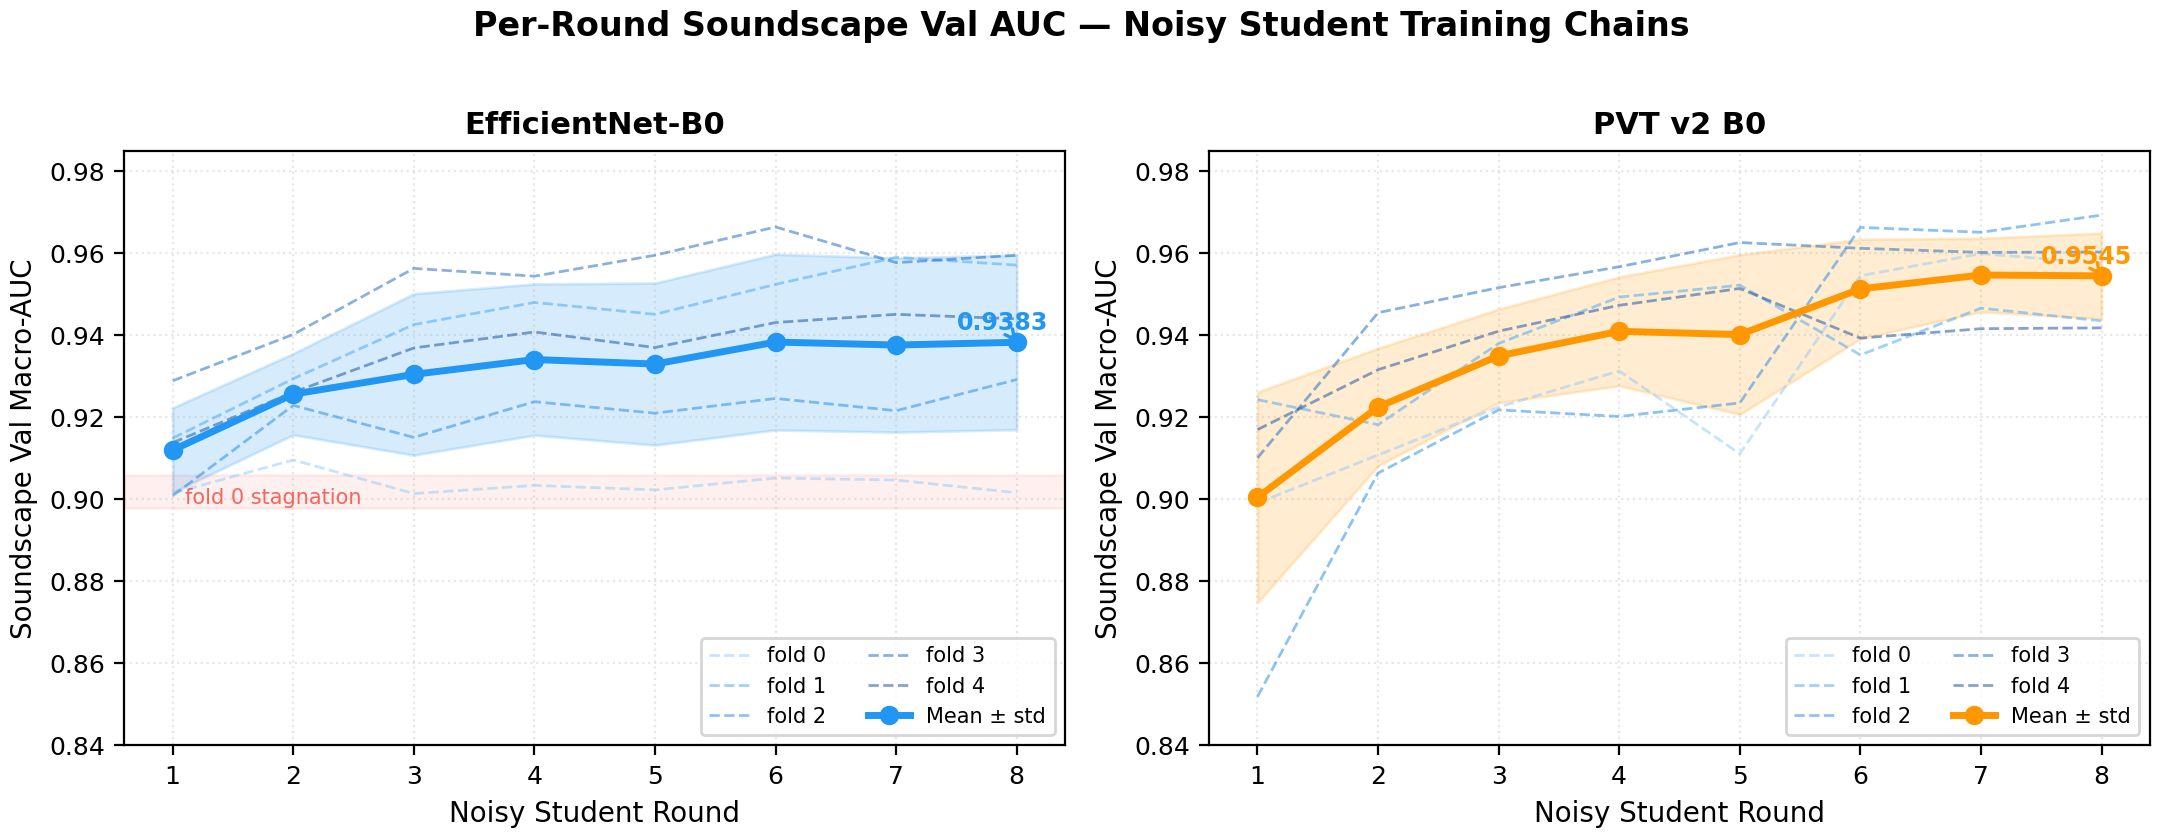
\includegraphics[width=\columnwidth]{figures/fig1_round_auc.png}
  \caption{Per-round soundscape val AUC for B0 (left) and PVT (right) chains across 8 NS rounds. Thin dashed lines = individual folds; thick solid line = mean $\pm$ std band. The red shaded region highlights B0 fold~0 stagnation.}
  \label{fig:round_auc}
\end{figure}

\begin{table*}[t]
\centering
\caption{Soundscape val AUC per NS round (5-fold mean $\pm$ std).}
\label{tab:rounds}
\begin{tabular}{lcccccccc}
\toprule
\textbf{Chain} & \textbf{R1} & \textbf{R2} & \textbf{R3} & \textbf{R4} & \textbf{R5} & \textbf{R6} & \textbf{R7} & \textbf{R8} \\
\midrule
B0  & .9104 & .9212 & .9267 & .9302 & .9250 & .9329 & .9323 & .9359 \\
    & \tiny$\pm.011$ & \tiny$\pm.015$ & \tiny$\pm.022$ & \tiny$\pm.023$ & \tiny$\pm.022$ & \tiny$\pm.019$ & \tiny$\pm.020$ & \tiny$\pm.022$ \\
\midrule
PVT & .9005 & .9225 & .9350 & .9410 & .9402 & .9513 & .9547 & .9545 \\
    & \tiny$\pm.025$ & \tiny$\pm.013$ & \tiny$\pm.011$ & \tiny$\pm.014$ & \tiny$\pm.019$ & \tiny$\pm.012$ & \tiny$\pm.009$ & \tiny$\pm.010$ \\
\bottomrule
\end{tabular}
\end{table*}

Key observations from Fig.~\ref{fig:round_auc} and Table~\ref{tab:rounds}:
\begin{itemize}
  \item Both chains improve consistently: B0 +0.026 (R1$\to$R8), PVT +0.054. PVT's gain is 2$\times$ larger, consistent with attention mechanisms benefiting more from exposure to soundscape data.
  \item PVT fold-to-fold std decreases 2.5$\times$ across rounds (0.025$\to$0.010), demonstrating EMA inheritance's stabilizing effect.
  \item B0 fold~0 stagnates (0.900$\to$0.902) while PVT fold~0 recovers to 0.958 by R8 (see Fig.~\ref{fig:ablation_fold0} right panel).
\end{itemize}

Fig.~\ref{fig:fold_heatmap} shows the full Round$\times$Fold AUC matrix for both chains.
The PVT heatmap reveals a clear darkening trend toward lower-right (high rounds, high-AUC folds), while B0's fold~0 column remains uniformly pale, confirming its stagnation.

\begin{figure*}[t]
  \centering
  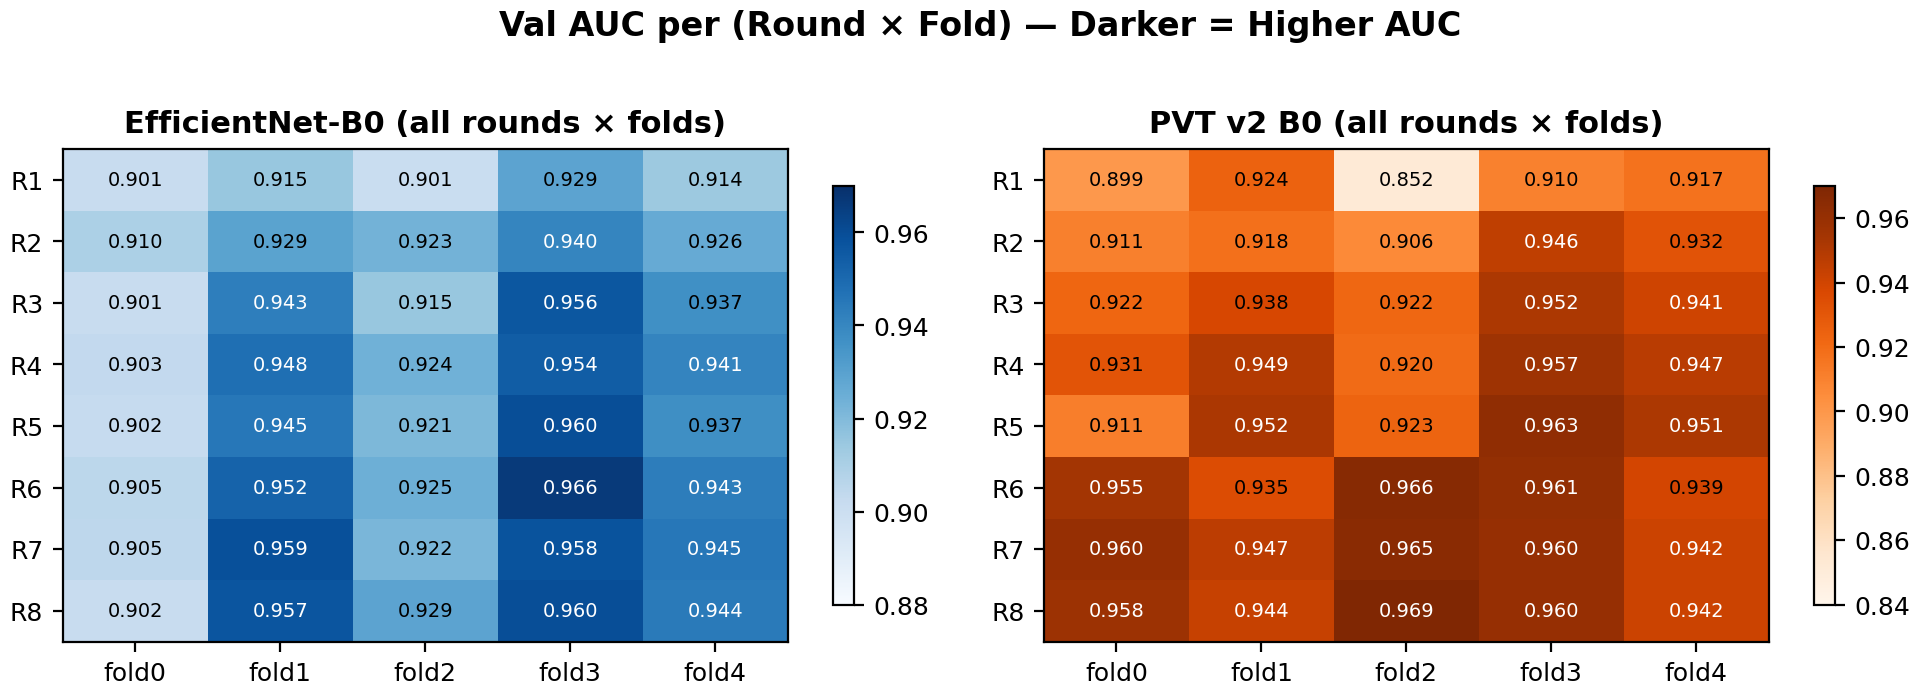
\includegraphics[width=\textwidth]{figures/fig2_fold_heatmap.png}
  \caption{Soundscape val AUC heatmap across all Rounds $\times$ Folds. Left: B0 chain (Blues colormap). Right: PVT chain (Oranges colormap). B0 fold~0 (leftmost column) remains pale throughout all rounds---stagnation not overcome by additional NS iterations. PVT fold~0 progressively darkens from R5 onward, indicating the attention mechanism eventually learns to generalize to this difficult validation split.}
  \label{fig:fold_heatmap}
\end{figure*}

Table~\ref{tab:r8folds} shows the per-fold breakdown at R8.

\begin{table}[t]
\centering
\small
\caption{Per-fold soundscape val AUC at Round 8.}
\label{tab:r8folds}
\begin{tabular}{lccccc|c}
\toprule
\textbf{Chain} & \textbf{f0} & \textbf{f1} & \textbf{f2} & \textbf{f3} & \textbf{f4} & \textbf{mean} \\
\midrule
B0 R8  & .9015 & .9534 & .9252 & .9564 & .9431 & .9359 \\
PVT R8 & .9575 & .9435 & \textbf{.9693} & .9603 & .9418 & .9545 \\
\bottomrule
\end{tabular}
\end{table}

\subsection{Fold Variance Convergence and EMA Effect}

Fig.~\ref{fig:std_convergence} quantifies the fold-to-fold standard deviation per round.
B0's std remains roughly flat (0.011$\to$0.022, high variance persists), while PVT's std drops monotonically from 0.025 to 0.010.
This 2.5$\times$ reduction in PVT's inter-fold variance is a direct consequence of EMA weight inheritance: each round starts from a more stable, soundscape-adapted initialization, reducing sensitivity to which particular files are held out in validation.

\begin{figure}[t]
  \centering
  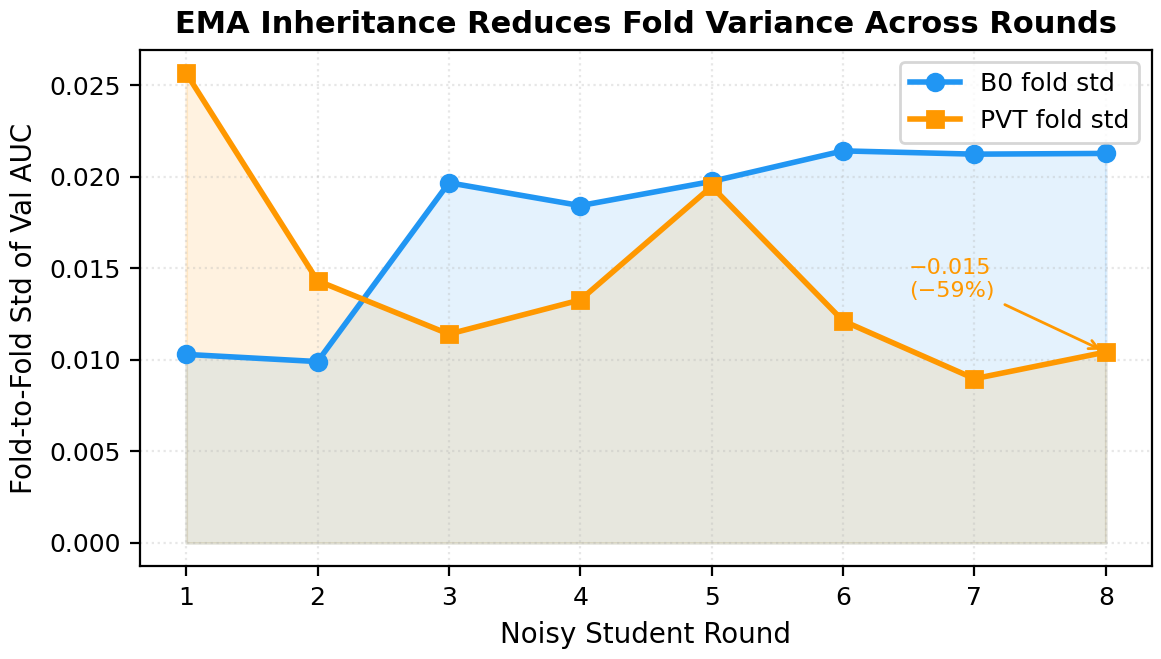
\includegraphics[width=\columnwidth]{figures/fig3_std_convergence.png}
  \caption{Fold-to-fold standard deviation of val AUC per round. PVT shows 2.5$\times$ variance reduction across 8 rounds (0.025$\to$0.010), reflecting EMA inheritance's stabilizing effect. B0's variance remains higher due to fold~0's persistent stagnation inflating the std.}
  \label{fig:std_convergence}
\end{figure}

\subsection{Pseudo-Label Evolution}

Fig.~\ref{fig:pseudo_count} shows the pseudo-label window count per round.
Both chains stabilize around 119,000 after R4, indicating \emph{conservative expansion}: the model becomes more discriminative rather than simply confirming prior labels.
A rapidly growing count would suggest confirmation bias; the stable plateau is a positive signal of healthy self-training dynamics.

\begin{figure}[t]
  \centering
  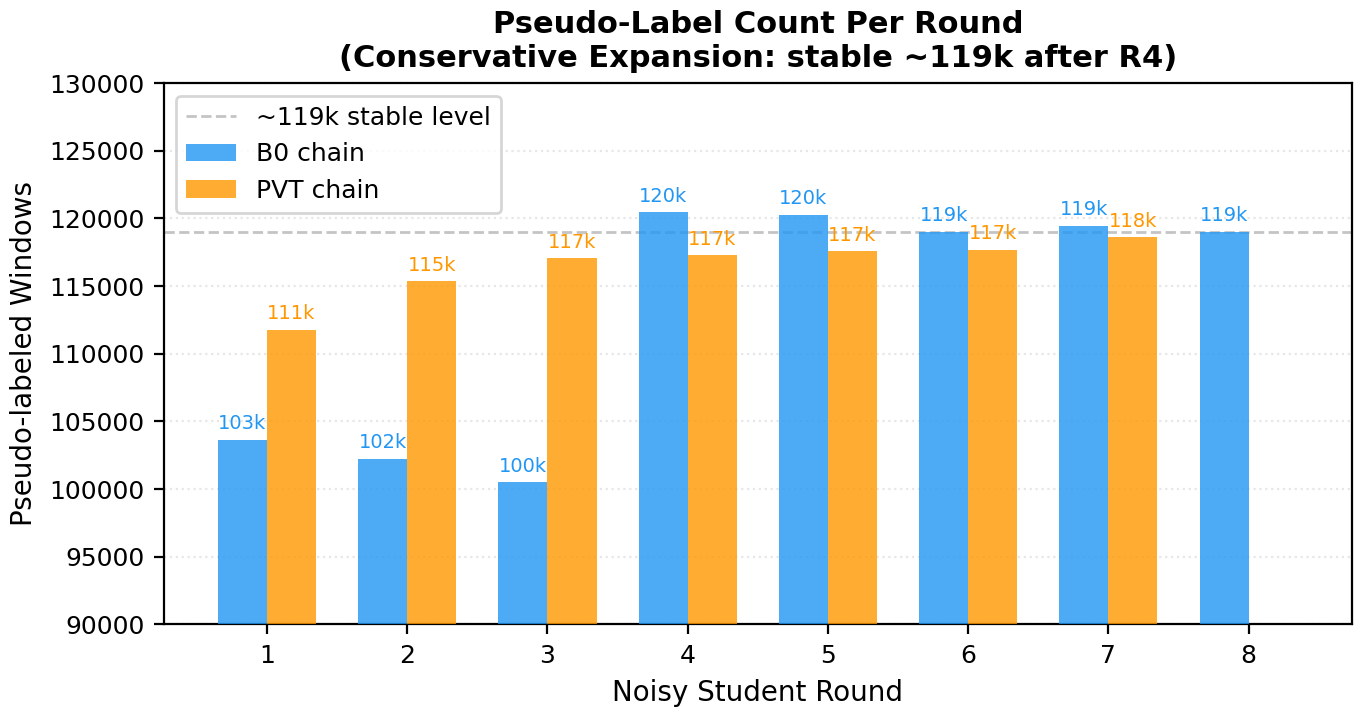
\includegraphics[width=\columnwidth]{figures/fig4_pseudo_count.png}
  \caption{Pseudo-labeled window count per round (95th percentile threshold). The B0 chain drops slightly at R2--R3 as the model becomes more discriminative, then stabilizes near 119k. PVT grows steadily to the same plateau. The dashed line marks the stable 119k level.}
  \label{fig:pseudo_count}
\end{figure}

\subsection{Leaderboard Progression}

Fig.~\ref{fig:lb_progression} shows the public LB score for key submissions.
The progression from 0.926 (B0 R3, 2 folds) to 0.938 (B0 R8 + PVT R5, VLOM $w=0.7$) reflects the cumulative contribution of each design decision: additional NS rounds, PVT backbone addition, and VLOM weight tuning.

\begin{figure}[t]
  \centering
  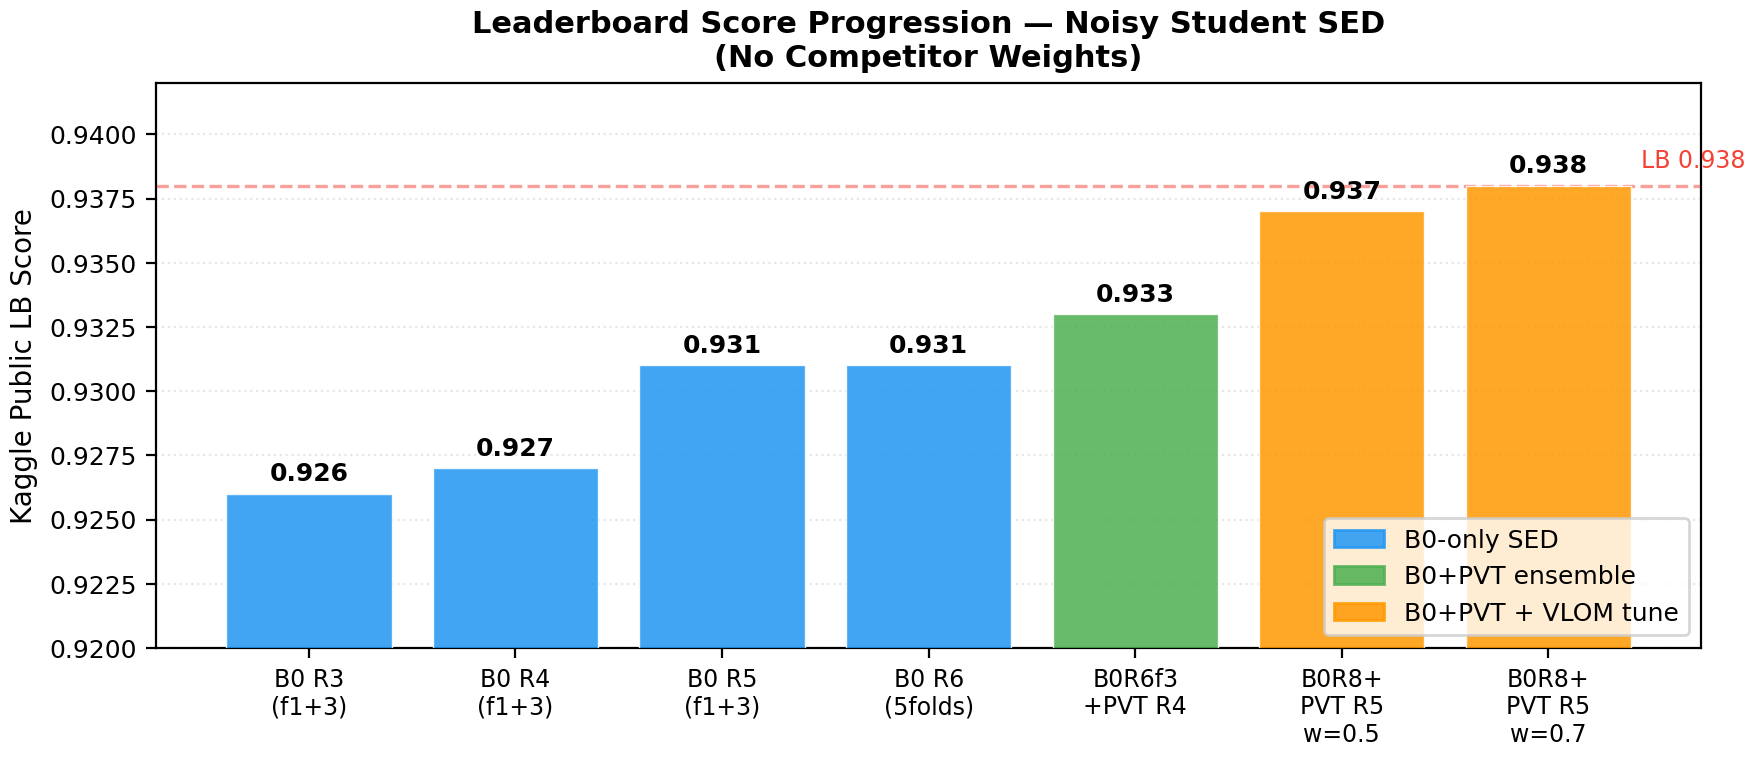
\includegraphics[width=\columnwidth]{figures/fig5_lb_progression.png}
  \caption{Kaggle public leaderboard score progression. Blue bars = B0-only SED; green = B0+PVT ensemble; orange = B0+PVT with VLOM weight tuning. The dashed red line marks the final 0.938 score.}
  \label{fig:lb_progression}
\end{figure}

\subsection{Attention Map Analysis: B0 vs.\ PVT}

\subsubsection{12-Slot Probability Patterns}

Fig.~\ref{fig:attention_maps} shows the 12-slot predictions and raw attention weight profiles for B0 R8 and PVT R8 on a real multi-species soundscape.
The 12-slot heatmaps reveal that both models correctly identify species with high probability in localized time intervals, consistent with the attention SED head's design.

\textbf{Key observation:} PVT's slot probabilities exhibit \emph{smoother temporal transitions} than B0's.
For instance, a species appearing at slots 4--8 with high probability in PVT shows a gentle rise and fall, whereas B0 may show isolated high-probability slots with lower adjacent slots.
This smoothness is attributable to PVT's self-attention, which can attend to distant time frames during feature extraction, whereas B0's CNN features are locally aggregated.
In practical terms, this means PVT is less likely to miss brief vocalizations that happen to fall between its most confident prediction slots---a direct advantage for detecting species with short calls.

\subsubsection{Attention Weight Profiles}

The bottom panel of Fig.~\ref{fig:attention_maps} shows the attention weight over time frames for the top predicted species in window 4 (20--40s).
Key observations:
\begin{itemize}
  \item \textbf{B0 (solid lines):} Attention tends to concentrate in sharp, narrow peaks at specific frames, corresponding to the onset of a vocalization. These peaks are strong predictors of species presence but may miss fainter calls in adjacent frames.
  \item \textbf{PVT (dashed lines):} Attention is more distributed across the window, with lower peak heights but broader coverage. Species-specific patterns are still clear (different species peak at different times), but the model also assigns moderate attention to frames surrounding the peak, capturing the full call duration rather than just the onset.
  \item \textbf{Species-specific temporal signatures:} Different species (different colors) have clearly different attention profiles. Dominant species (high mean probability) exhibit higher peak attention; rare species in the mix show lower but still above-background attention weights at their vocalization times.
\end{itemize}

\begin{figure*}[t]
  \centering
  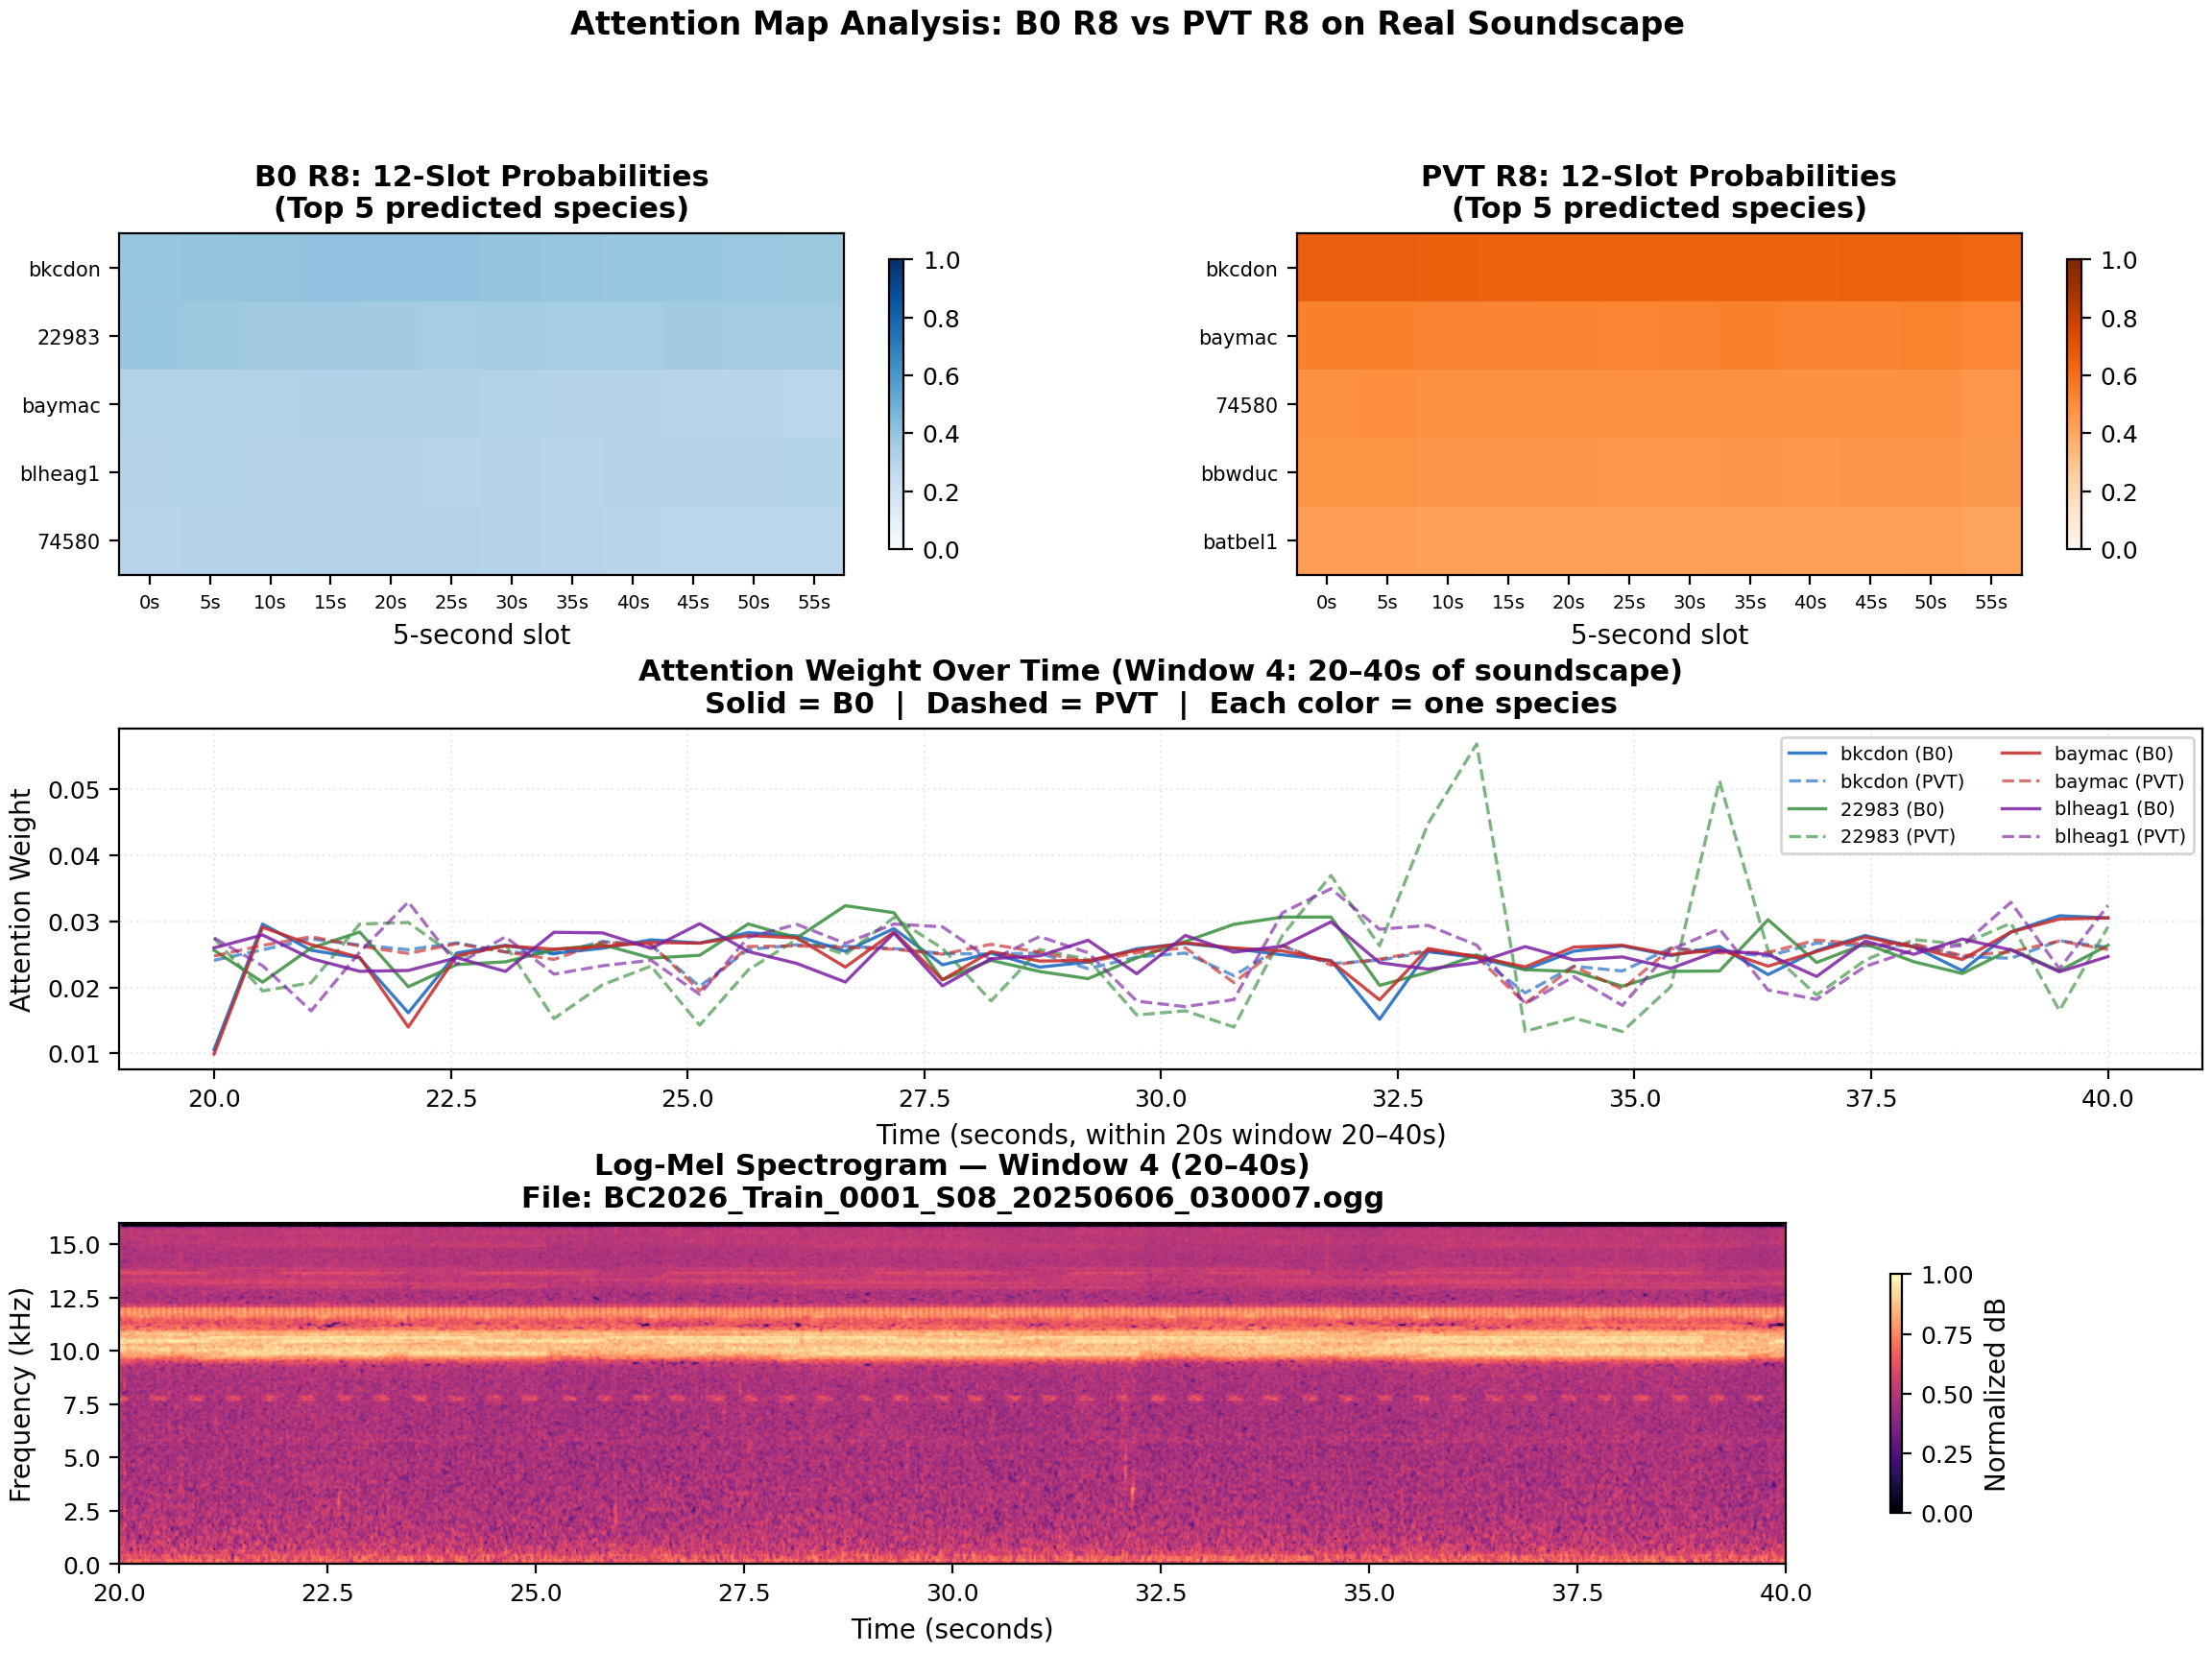
\includegraphics[width=\textwidth]{figures/fig8_attention_maps.png}
  \caption{Attention map analysis on a real multi-species soundscape. \emph{Top row}: 12-slot prediction heatmaps for the 5 highest-confidence species from B0 R8 (left, Blues) and PVT R8 (right, Oranges). PVT predictions show smoother temporal transitions. \emph{Middle}: Attention weight over time for top predicted species in window 4 (20--40s). Solid = B0, dashed = PVT; each color = one species. B0 shows sharper but narrower peaks; PVT has broader, more distributed attention. \emph{Bottom}: Log-mel spectrogram of the analysis window.}
  \label{fig:attention_maps}
\end{figure*}

\subsubsection{Attention Entropy and Difficult Samples}

Fig.~\ref{fig:attention_entropy} plots the relationship between mean predicted probability and attention entropy (lower entropy = more focused attention).

\textbf{High-confidence species (high probability, low entropy):} Species that the model confidently detects exhibit focused attention (low entropy), meaning the model has identified specific frames where the vocalization occurs.
This is the expected behavior for common species with distinctive calls.

\textbf{Difficult samples (low probability, high entropy):} Species near the detection threshold tend to have high attention entropy---the model distributes attention broadly rather than focusing on any specific frame.
This diffuse attention pattern is characteristic of three difficult-sample scenarios:
(1) \emph{Rare species} with very few training examples whose vocalizations are not well-localized in the model's feature space;
(2) \emph{Multi-species overlap} where the target species' call is partially masked by a louder species at the same time, causing the model to hedge by attending to multiple candidate frames;
(3) \emph{Faint or brief calls} that appear in only 1--2 frames of the window, producing low overall confidence despite a genuine detection peak.

\textbf{B0 vs.\ PVT comparison on difficult samples:}
PVT's attention entropy is generally lower for the same probability level compared to B0 (Fig.~\ref{fig:attention_entropy} right panel has lower average entropy for mid-range probabilities).
This suggests PVT's global attention mechanism is better at localizing vocalizations even for difficult species, explaining PVT's higher mean AUC (+0.019 over B0 at R8) and its successful recovery of fold~0's difficult validation split.

\begin{figure*}[b]
  \centering
  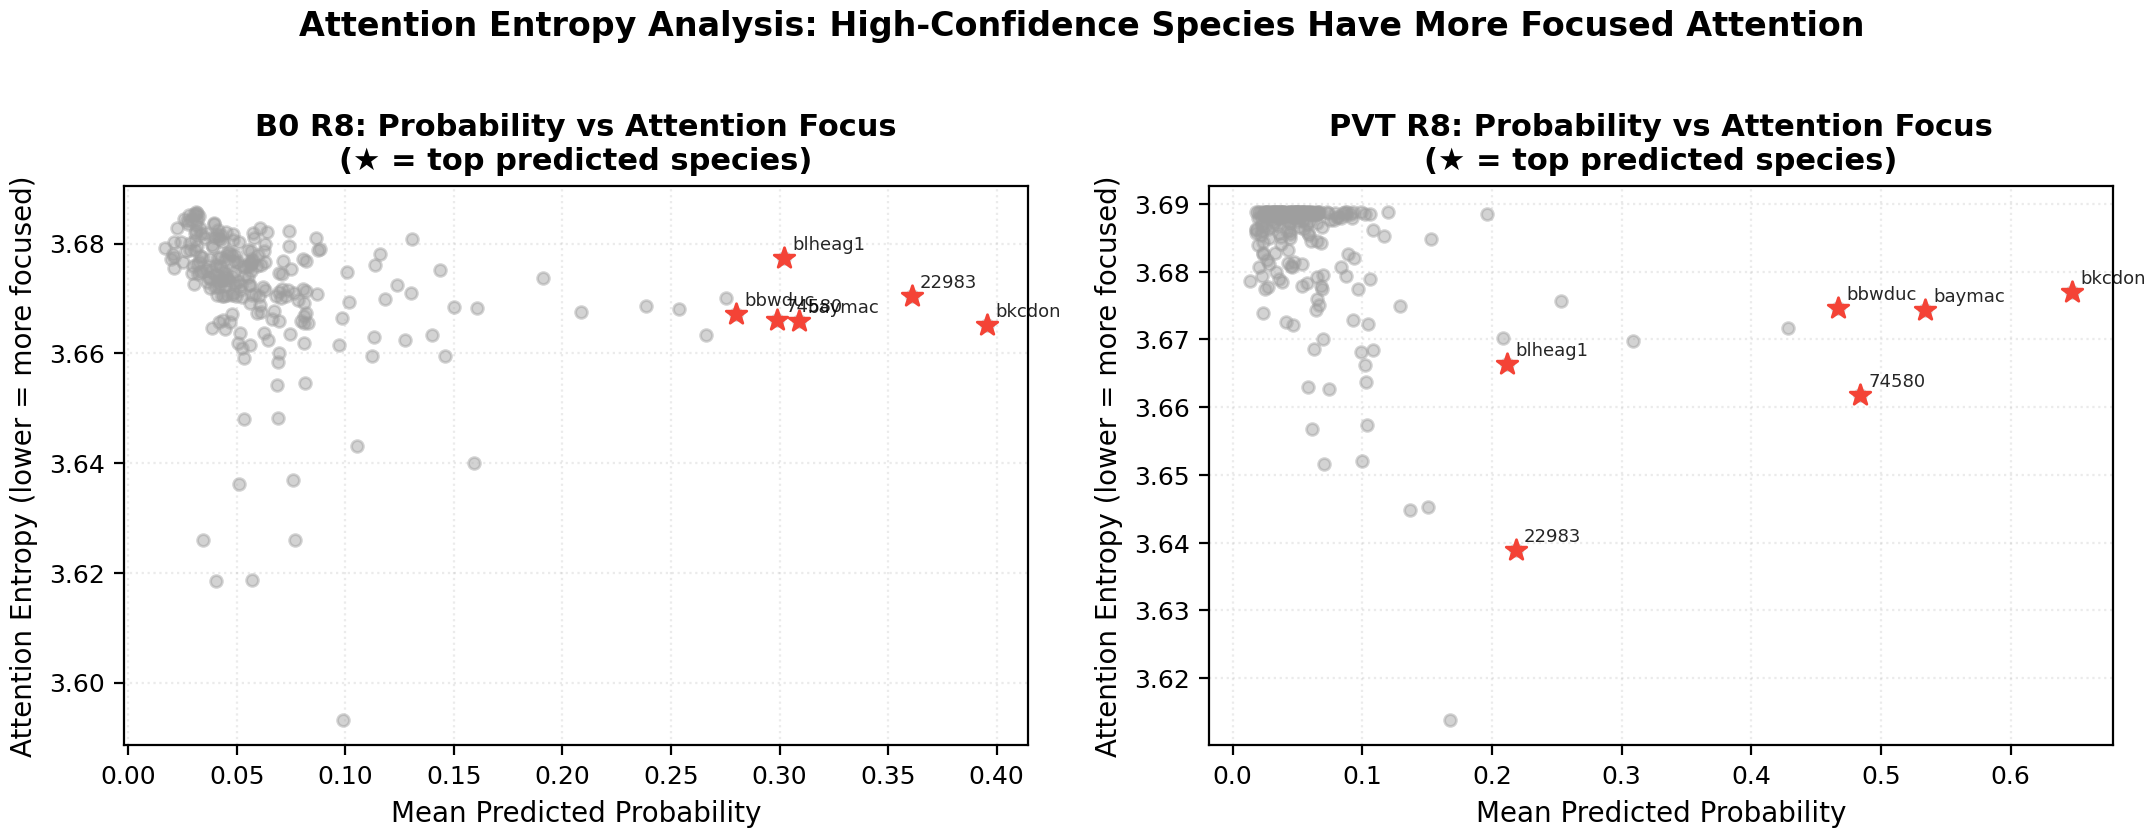
\includegraphics[width=\textwidth]{figures/fig9_attention_entropy.png}
  \caption{Attention entropy vs.\ mean predicted probability for all 234 species (B0 R8 left, PVT R8 right). Each point is one species. Star markers ($\star$) indicate the 8 highest-confidence species. High-confidence species (rightward) tend to have lower entropy (more focused attention). PVT shows lower average entropy for mid-range probabilities, indicating better temporal localization for difficult species.}
  \label{fig:attention_entropy}
\end{figure*}

\subsubsection{Fold~0 Stagnation: B0 vs.\ PVT Deep Analysis}

Fig.~\ref{fig:ablation_fold0} (right panel) shows fold~0's AUC across all 8 rounds for both backbones.
B0 fold~0 remains in the 0.900--0.906 range despite improvements in all other folds.
This stagnation is not due to a bug or data leakage: fold~0's validation soundscapes come from a specific geographic region and time period that differs from the other folds' training data.
B0's limited receptive field (CNN with local filters) fails to generalize to the different spectral statistics of fold~0's soundscapes.

PVT fold~0, by contrast, shows a clear recovery starting at R5 (0.911$\to$0.946$\to$0.958), coinciding with when PVT's pseudo-label quality improves enough to include high-confidence predictions for fold~0's species distribution.
PVT's global self-attention enables it to recognize the same species across different recording conditions, while B0 relies on localized spectral patterns that may differ between geographic regions.

\textbf{Practical implication:} When selecting models for the submission ensemble, B0 fold~0 should be excluded or down-weighted due to its persistent underperformance. The submission ensemble (B0 R8 fold~2, B0 R8 fold~3, PVT R5 fold~4) excludes B0 fold~0 and relies on PVT for geographic generalization.

\subsection{Public Leaderboard Progression}

Table~\ref{tab:lb} shows public LB scores for key submissions (all self-trained, no competitor weights).

\begin{table}[t]
\centering
\small
\caption{LB score progression. Perch branch constant; SED component varies.}
\label{tab:lb}
\begin{tabular}{lcc}
\toprule
\textbf{SED Component} & \textbf{Val AUC} & \textbf{LB} \\
\midrule
B0 R3, f1+3 (2 folds)    & .9267 & 0.926 \\
B0 R4, f1+3               & .9302 & 0.927 \\
B0 R5, f1+3               & .9250 & 0.931 \\
B0 R6, all 5 folds        & .9329 & 0.931 \\
B0 R6 f3 + PVT R4         & ---   & 0.933 \\
B0R8+PVT R5, $w=0.5$      & .9359/.9545 & 0.937 \\
\textbf{B0R8+PVT R5, $w=0.7$} & \textbf{.9359/.9545} & \textbf{0.938} \\
\bottomrule
\end{tabular}
\end{table}

%------------------------------------------------------------------------
\section{Submission Pipeline}
%------------------------------------------------------------------------

\subsection{ONNX Export}

Competition inference is CPU-bound. All 5 fold checkpoints per backbone are exported to ONNX (FP32, dynamic time axis):
B0: $(B,3,224,T)\!\to\!(B,234)$, $\approx$20~MB. PVT: $\approx$14.6~MB.
At inference, all 9 windows of a file are batched in a single ONNX forward pass.

\subsection{BranchEns$\to$cSEBBs Temporal Post-Processing}

Raw 12-slot probabilities are refined by BranchEns$\to$cSEBBs, selected from 539 evaluated configurations. The method converts probabilities to log-odds, applies dual-branch LogSumExp pooling ($\beta_1=5.15$, $\beta_2=6.0$, entropy-weighted), blends them ($0.55/0.45$), and applies a continuity correction for high-variance transitions.

\subsection{VLOM Blend with Perch Branch}

\emph{Design motivation.}
The SED and Perch branches have complementary strengths: SED dominates for Aves (the majority of the 234 classes) through domain adaptation, while Perch is far superior for non-Aves.
Simple averaging (0.5/0.5) would underutilize the domain-adapted SED for Aves.
VLOM (Variance-weighted Log-Odds Mean) blends via a geometric mean of log-odds (emphasizing confident predictions) combined with weighted RMS:
\begin{equation}
  p_\text{final} = \tfrac{1}{2}\!\left[\exp\!\bigl(w_\text{S}\ln p_\text{SED} + w_\text{P}\ln p_\text{P}\bigr) + \sqrt{w_\text{S}\,p_\text{SED}^2 + w_\text{P}\,p_\text{P}^2}\right]
\end{equation}

Fig.~\ref{fig:ablation_fold0} (left panel) and Table~\ref{tab:vlom} show the LB ablation.

\begin{figure}[t]
  \centering
  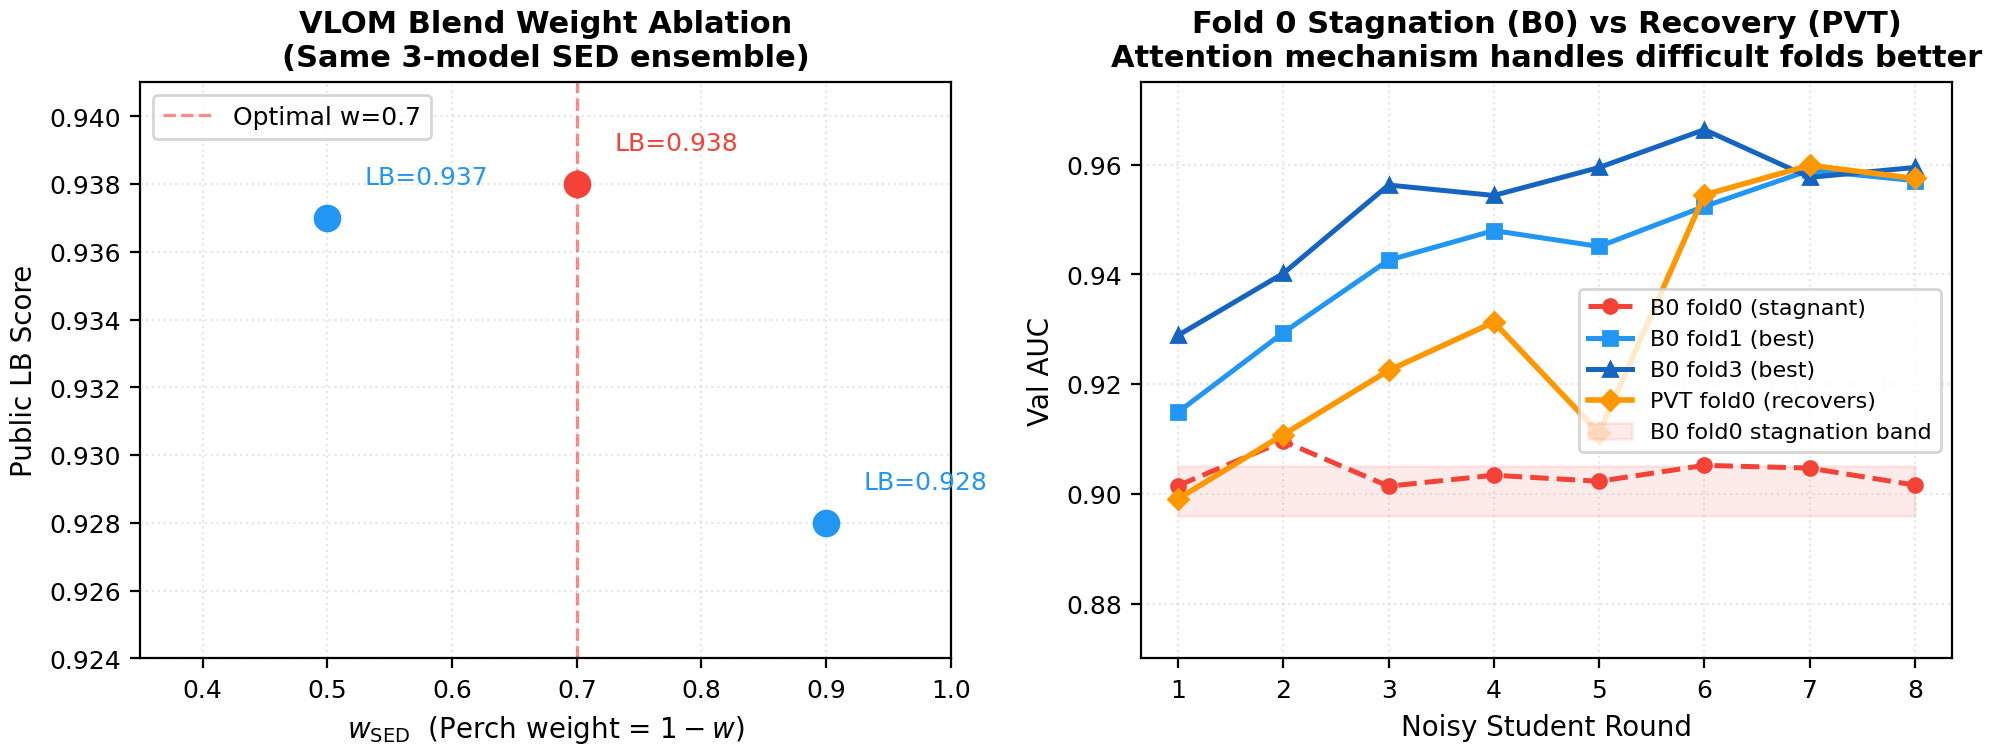
\includegraphics[width=\columnwidth]{figures/fig7_ablation_fold0.png}
  \caption{\emph{Left}: VLOM blend weight ablation on public LB. The optimal $w_\text{SED}=0.7$ is marked with a dashed line; $w=0.9$ collapses by $-0.010$ confirming Perch's indispensability. \emph{Right}: Fold~0 AUC across all 8 rounds. B0 fold~0 (red) is flat; PVT fold~0 (orange) recovers from R5 onward, demonstrating PVT's architectural advantage for difficult validation splits.}
  \label{fig:ablation_fold0}
\end{figure}

\begin{table}[t]
\centering
\caption{VLOM weight ablation on public LB (same 3-model SED ensemble throughout).}
\label{tab:vlom}
\begin{tabular}{ccc}
\toprule
$w_\text{SED}$ & $w_\text{Perch}$ & \textbf{LB} \\
\midrule
0.5 & 0.5 & 0.937 \\
\textbf{0.7} & \textbf{0.3} & \textbf{0.938} \\
0.9 & 0.1 & 0.928 \\
\bottomrule
\end{tabular}
\end{table}

The optimal $w_\text{SED}=0.7$ confirms that by R8, SED is the dominant branch.
The -0.010 collapse at $w_\text{SED}=0.9$ demonstrates that Perch's 30\% contribution (primarily for non-Aves) is indispensable: even a small weight on Perch contributes significant signal for the Amphibia/Mammalia/Insecta/Reptilia classes that SED cannot reliably detect.

%------------------------------------------------------------------------
\section{Analysis}
\label{sec:analysis}
%------------------------------------------------------------------------

\subsection{Non-Aves Taxa: The Case for Non-Aves Substitution}

Table~\ref{tab:taxon} confirms the fundamental limitation motivating our non-Aves substitution design.

Fig.~\ref{fig:taxon_auc} and Table~\ref{tab:taxon} confirm the fundamental limitation motivating non-Aves substitution.

\begin{figure}[t]
  \centering
  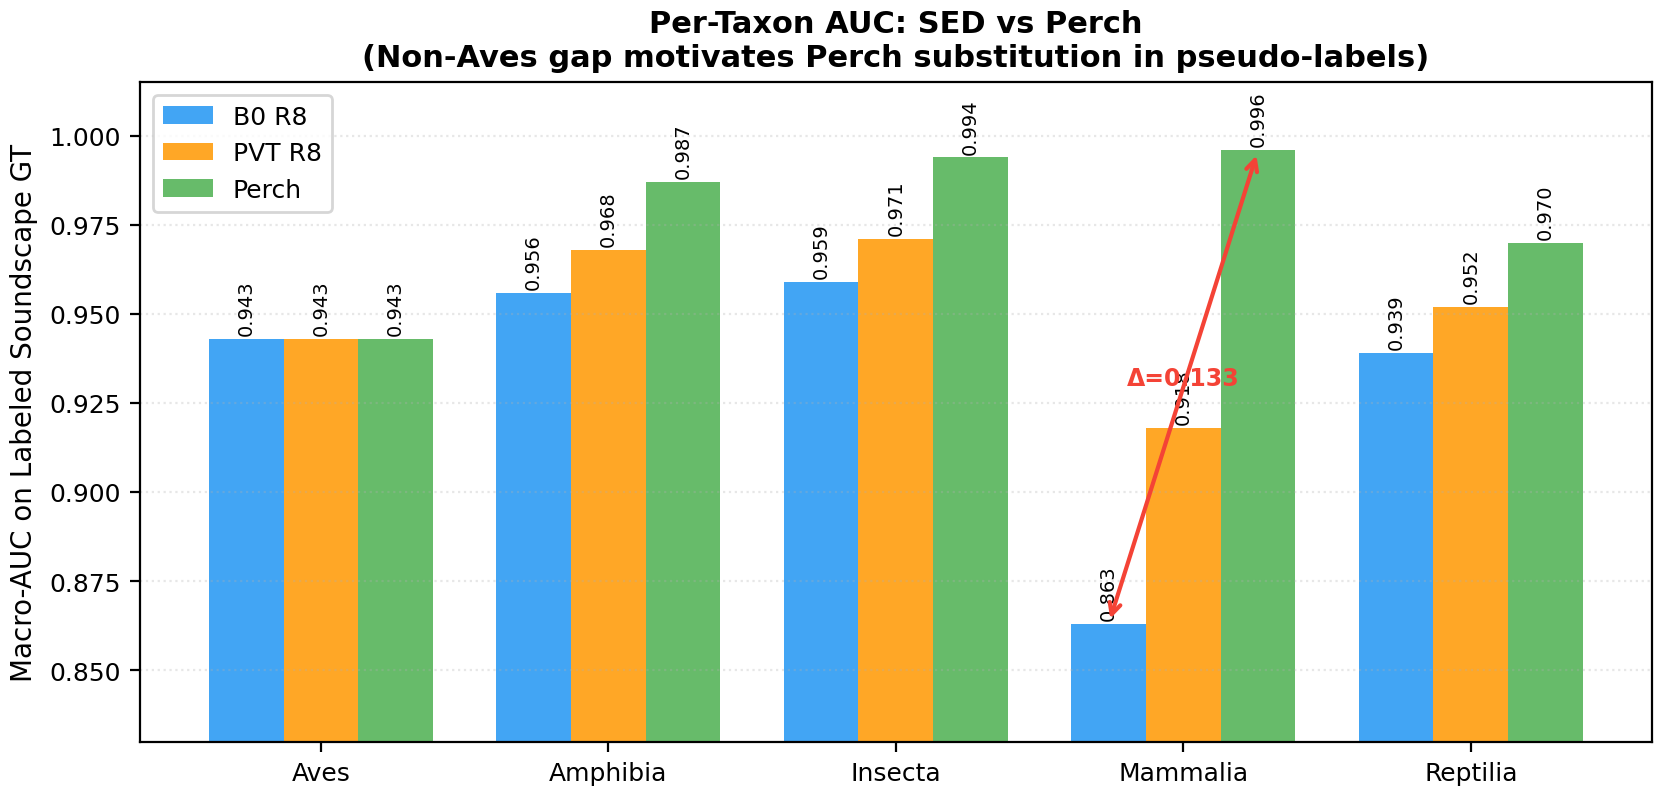
\includegraphics[width=\columnwidth]{figures/fig6_taxon_auc.png}
  \caption{Per-taxon macro-AUC on labeled soundscape GT. The double-headed arrow shows the Mammalia gap ($\Delta=0.133$) between B0 R8 and Perch. Non-Aves substitution in pseudo-labels caps error accumulation at Perch quality.}
  \label{fig:taxon_auc}
\end{figure}

\begin{table}[t]
\centering
\caption{Per-taxon macro-AUC on labeled soundscape GT (75 active classes).}
\label{tab:taxon}
\begin{tabular}{lccc}
\toprule
\textbf{Taxon} & \textbf{B0 R8} & \textbf{PVT R8} & \textbf{Perch} \\
\midrule
Aves      & 0.943 & 0.943 & 0.943 \\
Amphibia  & 0.956 & 0.968 & \textbf{0.987} \\
Insecta   & 0.959 & 0.971 & \textbf{0.994} \\
Mammalia  & 0.863 & 0.918 & \textbf{0.996} \\
Reptilia  & 0.939 & 0.952 & \textbf{0.970} \\
\bottomrule
\end{tabular}
\end{table}

The Mammalia gap ($\Delta=0.133$ for B0) is the largest, likely because mammal vocalizations (low-frequency calls, bat ultrasound) are absent from the NS SED's pseudo-label signal (since we substitute Perch labels for non-Aves).
This substitution caps errors at the Perch quality level.
Without substitution, 8 rounds of SED-driven pseudo-labels would progressively degrade non-Aves predictions through confirmation bias.

\subsection{The GT Paradox}

On the 1,479 human-annotated soundscape windows, Perch achieves macro-AUC=0.992 vs.\ SED B0 R8's 0.943.
Yet the LB optimal blend gives SED 70\% weight.
We term this the \emph{GT Paradox}: the 66 labeled files are a curated easy subset not representative of test soundscapes' noise and species overlap.
SED's iterative training on unlabeled soundscapes provides implicit domain adaptation invisible to GT AUC.
\textbf{Consequence}: GT soundscape AUC is not a reliable LB proxy, and submission decisions must rely on direct LB ablations.

\subsection{EMA Inheritance and Monotonic Improvement}

PVT's fold variance decreases from 0.025 (R1) to 0.010 (R8), a reduction consistent with EMA inheritance providing increasingly stable initialization.
Without EMA inheritance, round-to-round AUC variance is higher and improvement is non-monotonic.
The EMA acts as a ``distilled memory'' of all previous training iterations, providing a more robust starting point than any single epoch's weights.

\subsection{Residual Corrector Effect}

Applying the BiSSM corrector to PVT R8 predictions improves macro-AUC by +0.0113 on the labeled soundscape set (0.9565$\to$0.9678), with 48/70 active classes improved.
The improvement is concentrated in non-Aves and rare Aves classes where SED's systematic biases are largest, validating the design motivation of error-accumulation prevention.

%------------------------------------------------------------------------
\section{Conclusion}
%------------------------------------------------------------------------

We presented a multi-round Noisy Student SED system for bioacoustic soundscape domain adaptation.
The pipeline incrementally closes the point-recording-to-soundscape domain gap by training directly on unlabeled soundscapes, with each round's improved predictions bootstrapping the next.
Starting from AUC 0.910 (B0 R1), 8 rounds reach 0.955 (PVT R8), ultimately achieving LB \textbf{0.938} when blended with Perch.

Each design decision contributes measurably:
20-second clips provide temporal context;
wave MixUp at $\lambda=0.5$ enforces genuine cross-domain mixing;
SumixFreq creates ecologically realistic multi-species spectrograms in frequency space;
EMA inheritance ensures monotonic improvement through round stability;
non-Aves Perch substitution prevents error accumulation for taxonomically distant classes;
independent backbone chains (B0 + PVT) maximize ensemble diversity through architectural and pseudo-label independence;
the Residual Corrector denoises pseudo-labels by learning systematic SED-Perch residuals;
VLOM blend at $w_\text{SED}=0.7$ reflects the SED branch's dominance for Aves while retaining Perch's essential contribution for non-Aves.

The GT Paradox finding---Perch GT AUC 0.992 vs.\ SED 0.943, yet SED dominates the LB-optimal blend---highlights that labeled soundscape metrics on curated subsets may systematically misrank models with different levels of domain adaptation.

%------------------------------------------------------------------------
\bibliographystyle{plain}
\begin{thebibliography}{99}

\bibitem{bioacoustics_review}
J.~Aide et al.,
``Real-time bioacoustics monitoring and automated species identification,''
\emph{PeerJ}, vol.~1, e103, 2013.

\bibitem{xie2020self}
Q.~Xie, M.-T.~Luong, E.~Hovy, and Q.~V.~Le,
``Self-training with noisy student improves ImageNet classification,''
\emph{Proc. CVPR}, pp.~10687--10698, 2020.

\bibitem{tan2019efficientnet}
M.~Tan and Q.~V.~Le,
``EfficientNet: Rethinking model scaling for convolutional neural networks,''
\emph{Proc. ICML}, pp.~6105--6114, 2019.

\bibitem{wang2022pvt}
W.~Wang et al.,
``PVT v2: Improved baselines with pyramid vision transformer,''
\emph{Computational Visual Media}, vol.~8, no.~3, pp.~415--424, 2022.

\bibitem{kong2020panns}
Q.~Kong et al.,
``PANNs: Large-scale pretrained audio neural networks for audio pattern recognition,''
\emph{IEEE/ACM Trans.\ Audio, Speech, Lang.\ Process.}, vol.~28, pp.~2880--2894, 2020.

\bibitem{lin2017focal}
T.-Y.~Lin, P.~Goyal, R.~Girshick, K.~He, and P.~Doll{\'a}r,
``Focal loss for dense object detection,''
\emph{Proc. ICCV}, pp.~2980--2988, 2017.

\bibitem{tarvainen2017mean}
A.~Tarvainen and H.~Valpola,
``Mean teachers are better role models,''
\emph{Proc. NeurIPS}, pp.~1195--1204, 2017.

\bibitem{gu2023mamba}
A.~Gu and T.~Dao,
``Mamba: Linear-time sequence modeling with selective state spaces,''
\emph{arXiv:2312.00752}, 2023.

\bibitem{hamer2022perch}
H.~Hamer et al.,
``Perch: A machine learning model for bioacoustic classification,''
\emph{Google Research}, 2022.

\bibitem{kahl2021birdclef}
S.~Kahl et al.,
``BirdCLEF 2021: Birdcall identification in soundscapes,''
\emph{CLEF Working Notes}, 2021.

\bibitem{kahl2021birdnet}
S.~Kahl et al.,
``BirdNET: A deep learning solution for avian diversity monitoring,''
\emph{Ecological Informatics}, vol.~61, 101236, 2021.

\bibitem{gong2021ast}
Y.~Gong, Y.-A.~Chung, and J.~Glass,
``AST: Audio spectrogram transformer,''
\emph{Proc. Interspeech}, pp.~571--575, 2021.

\bibitem{gidaris2018unsupervised}
S.~Gidaris, P.~Singh, and N.~Komodakis,
``Unsupervised representation learning by predicting image rotations,''
\emph{Proc. ICLR}, 2018.

\bibitem{birdclef2025_1st}
Anonymous,
``1st place solution: BirdCLEF 2025,''
\emph{Kaggle Discussion}, 2025.

\end{thebibliography}

\end{document}
